\section{exec}

	Ejecute los programas: fork-execl.c, fork-execlp.c, fork-execv.c, fork-execvp.c. Muestre la pantalla de ejecucución del programa:

	\begin{center}
		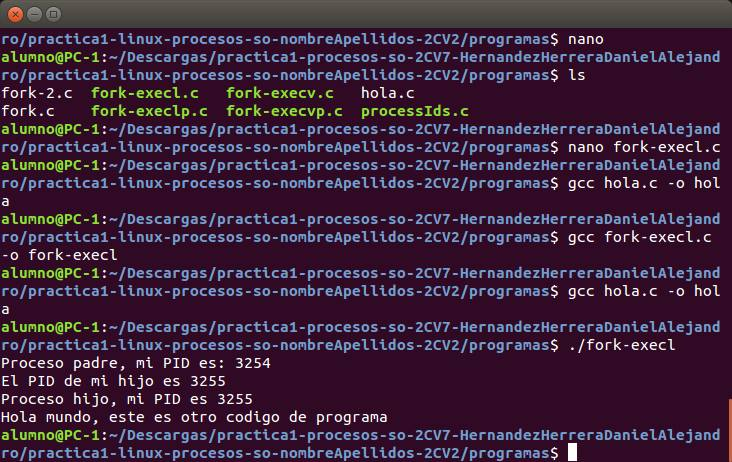
\includegraphics[width=\linewidth]{imagenes/execl.png}
		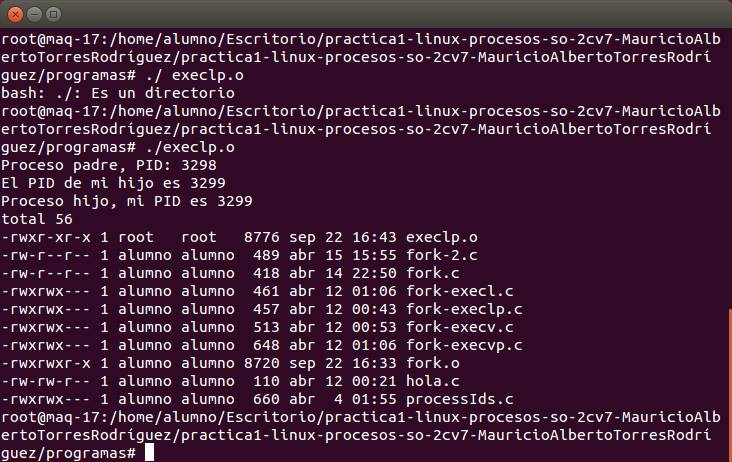
\includegraphics[width=\linewidth]{imagenes/execlp.png}
		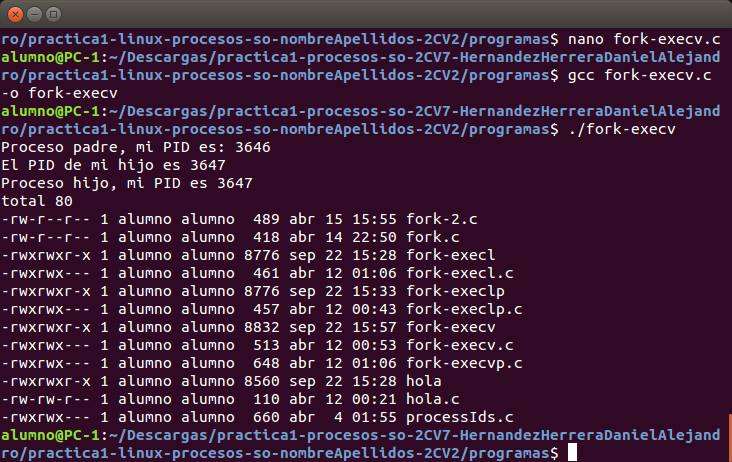
\includegraphics[width=\linewidth]{imagenes/execv.png}
		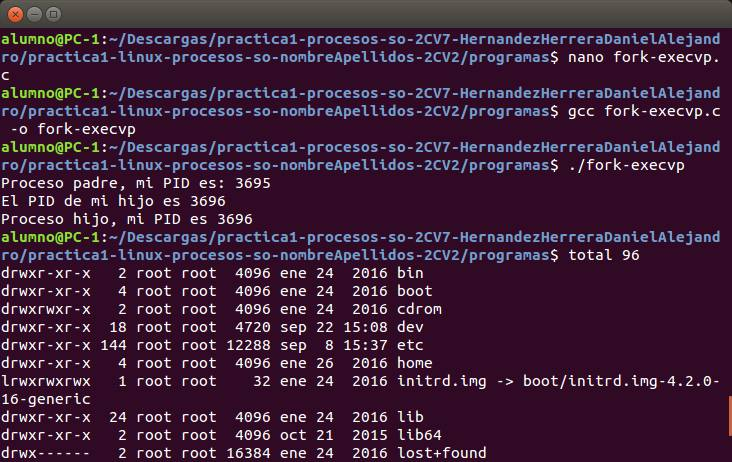
\includegraphics[width=\linewidth]{imagenes/execvp.png}
	\end{center}

	Investigue para que se ocupa la familia de funciones exec y describa para cada función su utilidad y argumentos de entrada:
\\ \\
\textbf{La familia exec...()} es un conjunto de funciones que en esencia realizan la misma actividad ya que solo difieren en la forma de pasar sus argumentos, son utilizadas para poner en ejecución un proceso determinado, la característica es que las instrucciones del proceso que las invoca son sustituidas por las instrucciones del proceso indicado. 
\\ \\
Si la llamada falla se retornara -1.
\\ \\
Para su funcionamiento se requiere incluir el archivo de cabecera: unistd.h
\\ \\
	\textbf{Nombres en la familia exec.}
\\ La familia de funciones exec utiliza letras como sufijos para indicar los parámetros que requieren y su comportamiento: 
\\ \\ p: Buscan la ruta del programa 
\\ l: Los parámetros se pasan separados por comas 
\\ v: Los parámetros se pasan en un vector 
\\ e: Una matriz de punteros a la configuración de entorno, se pasa al nuevo proceso.


	\begin{itemize}

		\item execl
\\ - Nombre y ruta del fichero ejecutable. 
\\ - Ristras separadas por comas con cada uno de los argumentos. 
\\ Ejemplo: 
\\ extern const char* environ[]; execl("/bin/ls", "/bin/ls", "-l", (const char *)NULL);

		\item execlp
\\ - Nombre del fichero ejecutable (implementa búsqueda del programa). 
\\ - Ristras separadas por comas con cada uno de los argumentos. 
\\ Ejemplo: 
\\ extern const char* environ[]; execlp("ls", "ls" , "-l", (const char *)NULL);

		\item execv
\\ - Nombre y ruta del fichero ejecutable. 
\\ - Vector de ristras de caracteres con los argumentos. 
\\ Ejemplo:
\\ extern const char* environ[]; char *argv[] = {"-l", (const char*)NULL}; execv("/bin/ls", argv);

		\item execvp
\\ - Nombre del fichero ejecutable (implementa búsqueda del programa). 
\\ - Vector de ristras de caracteres con los argumentos. 
\\ Ejemplo: 
\\ extern const char* environ[]; char *argv[] = {"-l", (const char*)NULL}; execv("ls", argv);

		\item execle	
\\ - Nombre y ruta del fichero ejecutable. 
\\ - Ristras separadas por comas con cada uno de los argumentos. 
\\ - Vector de ristras de caracteres con las variables de entorno y sus valores. 
\\ Ejemplo:
\\ char *env[] = {"PATH=/bin", (const char*)NULL}; execle("/bin/ls", "/bin/ls", "-l", (const char *)NULL, env);

		\item execve
\\ - Nombre (y ruta) del programa 
\\ - Lista de parámetros que se pasarán al programa 
\\ - Lista de variables de entorno y sus valores
\\ Ejemplo: 
\\ execve(const char *filename, char *const argv[], char *const envp[]);

	\end{itemize}
